\documentclass[UTF8,zihao=-4]{ctexart}
\usepackage[a4paper,margin=2.5cm]{geometry}
\usepackage{amsmath, amssymb, amsthm}
\usepackage{bm}
\usepackage{hyperref}
\usepackage{graphicx}
\usepackage{caption}
\usepackage{listings}
\usepackage{xcolor}
\usepackage{float}
\usepackage{booktabs}
\usepackage{longtable}
\usepackage{multirow}
\usepackage{placeins}
\graphicspath{{figures/}}

% 代码样式
\lstdefinestyle{code}{
  basicstyle=\ttfamily\small,
  numbers=left,
  numberstyle=\tiny,
  numbersep=8pt,
  keywordstyle=\color{blue},
  commentstyle=\color{teal!70!black},
  stringstyle=\color{orange!70!black},
  showstringspaces=false,
  breaklines=true,
  frame=single,
  framerule=0.3pt,
  rulecolor=\color{black!15}
}
\lstset{style=code}

\title{迈向自治智能:世界模型、持续学习与跨学科应用}
\author{}
\date{\today}

\begin{document}
\maketitle

\section{World Model 与 Memory-Augmented LM}
\subsection{整体框架}
世界模型(World Model)尝试对环境动态进行显式建模,使语言模型能够“想象”未来状态,再配合记忆增强(Memory-Augmented)机制形成闭环。图\ref{fig:world_model_pipeline_cn} 展示了从感知输入到策略生成的典型流水线:原始数据通过世界模型抽象成潜空间,再结合长短期记忆,以语言模型/策略模块做决策与交互。
\begin{figure}[H]
  \centering
  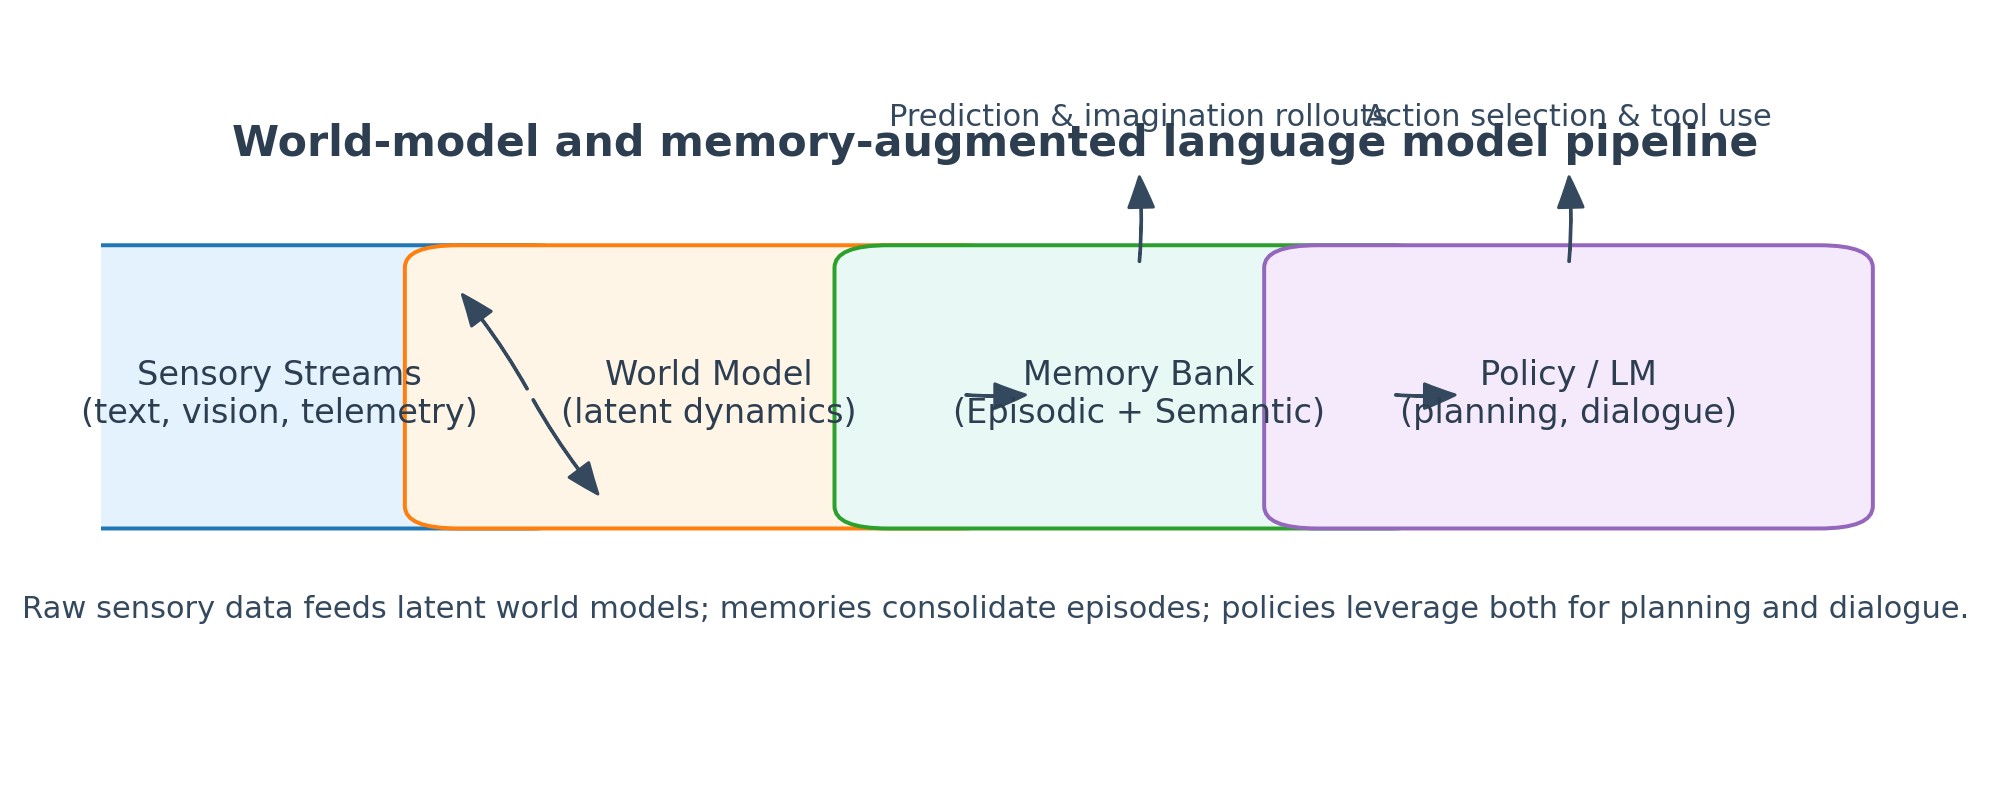
\includegraphics[width=0.95\textwidth]{world_model_pipeline.png}
  \caption{世界模型 + 记忆增强 LLM 流水线:感知 \textrightarrow{} 世界模型 \textrightarrow{} 记忆库 \textrightarrow{} 策略/语言模型。}
  \label{fig:world_model_pipeline_cn}
\end{figure}

\subsection{世界模型核心要素}
\begin{itemize}
  \item \textbf{潜变量建模:} 通过 VAE、Transformer 状态空间模型(e.g., Dreamer、TD-MPC)建立状态表示;
  \item \textbf{预测与反事实推演:} 进行 imagination rollout,帮助模型评估长远后果;
  \item \textbf{模型-环境对齐:} 结合真实交互数据与模型生成数据,避免分布漂移。
\end{itemize}

\subsection{记忆增强策略}
\begin{itemize}
  \item \textbf{工作记忆(Working Memory):} 用于当前任务的临时上下文,常采用 KV Cache、外部缓冲;
  \item \textbf{情景记忆(Episodic Memory):} 记录事件序列,可通过向量数据库检索历史片段;
  \item \textbf{语义记忆(Semantic Memory):} 存储长期知识或技能树,利于跨任务迁移;
  \item \textbf{记忆管理:} 包括写入策略、遗忘/压缩、优先级排序、冲突解决。
\end{itemize}

\section{Self-Improving 与 Continual Learning}
\subsection{自我改进循环}
自我改进(Self-Improving)强调模型在运行中不断评估并修正自身,可概括为:
\begin{enumerate}
  \item \textbf{自监督观察:} 收集推理日志、用户反馈、失败样本;
  \item \textbf{自我诊断:} 利用辅助模型评估性能、定位错误类型;
  \item \textbf{自我更新:} 通过经验回放、梯度更新、权重平均(EMA)或增量微调更新模型;
  \item \textbf{验证与回滚:} 在线/离线测试通过后再滚动发布,保留回滚策略。
\end{enumerate}

\subsection{持续学习(Continual Learning)方法}
\begin{itemize}
  \item \textbf{参数正则:} EWC、SI、L2P 约束新任务更新,避免灾难性遗忘;
  \item \textbf{经验回放:} 保留代表性样本或合成数据(Generative Replay);
  \item \textbf{模块化架构:} 通过适配器、LoRA、专家网络为新任务增量扩展;
  \item \textbf{任务检测:} 利用分布漂移监控自动识别新任务、触发自适应流程。
\end{itemize}

\subsection{评估指标}
\begin{itemize}
  \item \textbf{累积性能:} 新旧任务平均准确率;
  \item \textbf{遗忘程度:} 与初始任务性能差值;
  \item \textbf{学习效率:} 单任务训练时间、梯度步数、能源消耗;
  \item \textbf{稳定-可塑性平衡:} 衡量新知识吸收与旧知识保持的 trade-off。
\end{itemize}

\section{Agentic Systems(MetaGPT, Voyager)}
\subsection{代表系统解析}
图\ref{fig:agentic_ecosystem_cn} 总结了以 MetaGPT、Voyager 为代表的 Agentic 系统与配套基础设施:角色规划、开放世界探索、自我改进循环、记忆设施、持续学习管道以及科学场景落地构成生态闭环。
\begin{figure}[H]
  \centering
  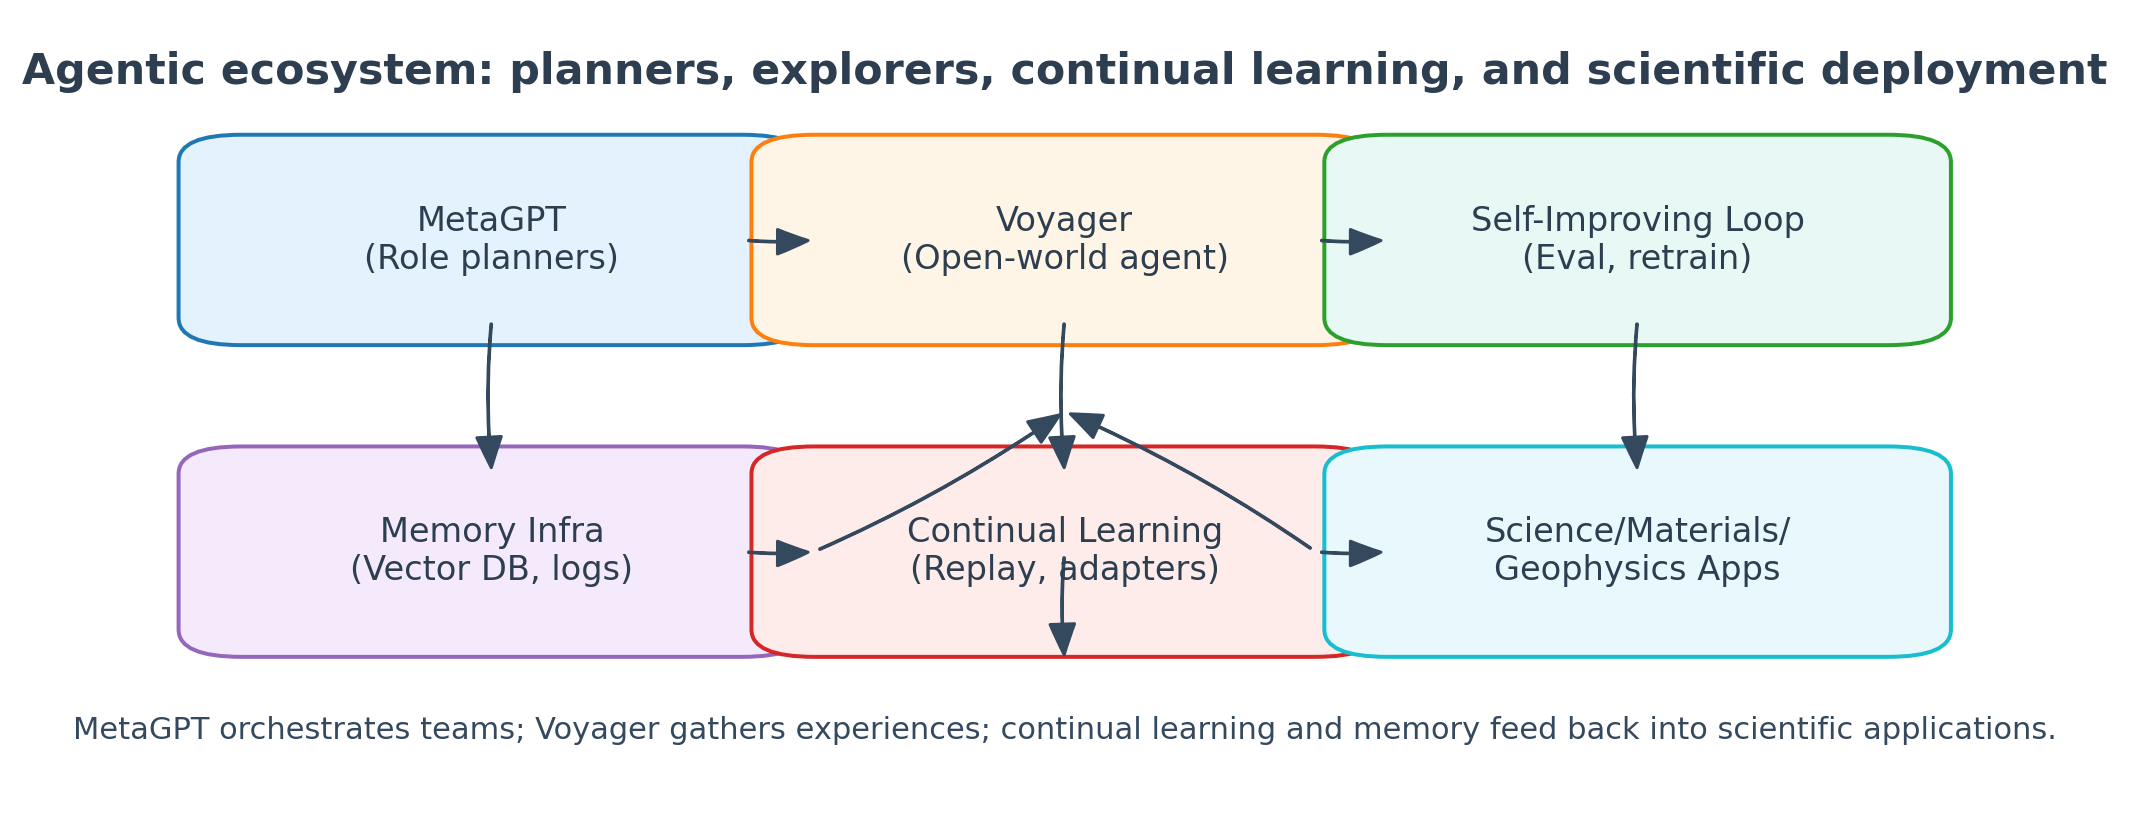
\includegraphics[width=0.95\textwidth]{agentic_ecosystem.png}
  \caption{Agentic 生态:MetaGPT(角色规划)、Voyager(开放世界探索)、持续学习、跨学科应用闭环。}
  \label{fig:agentic_ecosystem_cn}
\end{figure}

\subsection{MetaGPT}
\begin{itemize}
  \item \textbf{角色分工:} 预设 PM、架构师、工程师、QA 等角色,由 LLM 扮演;
  \item \textbf{任务流水线:} 需求分析、设计文档、代码生成、测试验证自动衔接;
  \item \textbf{记忆共享:} 通过知识库和任务板(Task Board)协调多智能体协作;
  \item \textbf{应用场景:} 软件开发、数据分析、文案创作等团队型工作流。
\end{itemize}

\subsection{Voyager}
\begin{itemize}
  \item \textbf{开放世界学习:} 在 Minecraft 等环境中自主探索、发现工具;
  \item \textbf{技能库:} 将成功策略保存为技能函数,按需检索复用;
  \item \textbf{自我改进:} 失败后分析原因,迭代 prompt 与代码,形成 self-learning;
  \item \textbf{扩展:} 支持多环境(机器人、模拟器),结合世界模型与规划器。
\end{itemize}

\subsection{Agentic 系统设计要点}
\begin{itemize}
  \item 角色体系与权限管理(Role-based access control);
  \item 记忆层次化:情景记忆 + 语义记忆 + 工具记忆;
  \item 弹性自我改进:可插拔的评估器、调优管道;
  \item 安全治理:操作审计、异常回滚、人类监督。
\end{itemize}

\section{AI for Science / Materials / Geophysics 应用前景}
\subsection{科学研究中的自治智能}
\begin{itemize}
  \item \textbf{科研流程自动化:} 自动文献综述、假设生成、实验设计、数据分析;
  \item \textbf{实验机器人:} 与实验设备对接,执行自动实验、收集数据并反馈给模型;
  \item \textbf{数据管理:} 统一实验日志、传感器数据、模拟结果,形成知识图谱。
\end{itemize}

\subsection{材料科学}
\begin{itemize}
  \item \textbf{生成式设计:} 利用世界模型预测材料性质,结合贝叶斯优化筛选候选材料;
  \item \textbf{多尺度模拟:} 将分子动力学、量子化学、宏观模拟结果融入统一记忆;
  \item \textbf{闭环实验:} 设计-合成-表征-分析形成自治循环,加速新材料发现。
\end{itemize}

\subsection{地球物理与能源}
\begin{itemize}
  \item \textbf{反演与预测:} 结合地震、地磁、遥感数据构建世界模型,提高地质结构解释精度;
  \item \textbf{风险评估:} 自动识别异常事件(地震、火山、滑坡)并给出应急预案;
  \item \textbf{碳捕集与储存:} 优化监测网络、模拟地下储层演化,提高 CCS 项目安全性。
\end{itemize}

\subsection{挑战与展望}
\begin{itemize}
  \item 数据共享与隐私合规,跨机构协同;
  \item 多模态融合与高维物理约束;
  \item 人机协同:确保科学家可理解、可控制自治系统;
  \item 伦理与治理:避免错误决策带来重大损失,建立审计机制。
\end{itemize}

\section*{实践建议}
\begin{itemize}
  \item 在架构设计上将世界模型、记忆模块、评估器解耦,便于迭代与扩展;
  \item 构建自我改进流水线:数据收集、标签校验、实验验证、模型更新;
  \item 对 Agentic 系统强化安全与合规审查,引入人类在环(HITL)机制;
  \item 与科研团队合作,建立跨学科基准与实验平台,加速 AI for Science 落地。
\end{itemize}

\section*{参考文献}
\begin{itemize}
  \item Ha and Schmidhuber. ``World Models.'' NeurIPS, 2018.
  \item Hafner et al. ``DreamerV3: Mastering Diverse Domains via World Models.'' arXiv, 2023.
  \item Hong et al. ``MetaGPT: Meta Programming for Multi-Agent Collaborative Framework.'' arXiv, 2023.
  \item Wang et al. ``Voyager: An Open-Ended Embodied Agent with LLMs.'' arXiv, 2023.
  \item AI4Science Community. ``Autonomous Discovery in Materials and Chemistry.'' Nature, 2024.
\end{itemize}

\end{document}

